\documentclass[main.tex]{subfiles}
\begin{document}
\chapter{Mechanics}
\section{Scalars and Vectors}
\spec{(a) distinguish between scalar and vector quantities and give examples of each}
A scalar quantity\footnote{strictly we are modelling a physical quantity as a mathematical object} is one which has only a magnitude whereas a vector has \emph{both} magnitude and direction. We often use positive and negative values to indicate direction (e.g. $v=-2\ ms^{-1}$) but this does not mean that all negative values are vectors!

Note that there are different ways of multiplying vectors and scalars. Two vectors can be multiplied to give a scalar \emph{or} a vector. For example, word done is the (scalar) product of force and displacement, both vectors.

\spec{(b) resolve a vector into two components at right angles to each other by drawing and by calculation}

Vectors can be split into two components using trigonometry. The diagram below shows a velocity vector being split into horizontal and vertical components $v_x$ and $v_y$.

\begin{figure}[h]
\begin{center}
\begin{tikzpicture}
	\draw[very thick, black, ->] (0,0) -- node[above] {$\mathbf{v}$}  (5,2.5);
	\draw[very thick, purple, ->] (0,0) -- node[below] {$\mathbf{v_x}$} (5,0);
	\draw[very thick, purple, ->] (0,0) -- node[left]{$\mathbf{v_y}$}(0,2.5);
	\draw [very thick,gray](1,0) arc (0:26.6:1);
	\draw [gray](1,0.25) node[right]{$\theta$};
	\draw (7,1.25) node[right] {
		$\begin{aligned}
		\mathbf{v}&=\mathbf{v_x + v_y}\\
		v_x &= v\cos{\theta}\\
		v_y &= v\sin{\theta}
		\end{aligned}$};
\end{tikzpicture}
\end{center}
\end{figure}

\spec{(c) combine any number of coplanar vectors at any angle to each other by drawing}

Vectors can be added by placing them end to end. The resultant vector is the one joining the start of the first vector to the end of the final vector. Its magnitude and direction can be calculated by trigonometry or scale drawing.

\begin{figure}[h]
	\begin{center}
	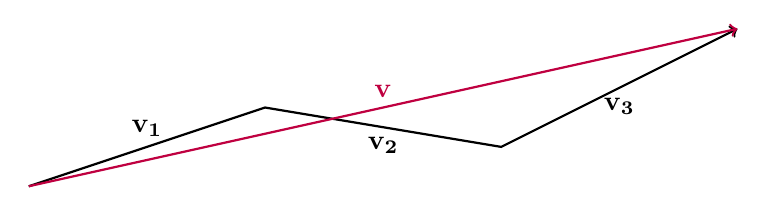
\begin{tikzpicture}
	\draw[thick,->] (0,0) -- node[above] {$\mathbf{v_1}$} (3,1) -- node[below] {$\mathbf{v_2}$} (6,.5) -- node[below] {$\mathbf{v_3}$} (9,2);
	\draw[thick,purple,->] (0,0) -- node[above]{$\mathbf{v}$} (9,2);
	\end{tikzpicture}
	$$\mathbf{v} = \mathbf{v_1}+\mathbf{v_2}+\mathbf{v_3}$$
	\end{center}
\end{figure}

\section{Forces and Accelerations}

\spec{(d) calculate the moment of a force and use the conditions for equilibrium to solve problems (restricted to
	coplanar forces)}

The moment of a force is calculated by multiplying its magnitude by the perpendicular distance of the force's line of action to the pivot point. This is mathematically equivalent to multiplying the distance from the pivot by the component of the force perpendicular to that distance.

\begin{figure}[h]
	\centering
	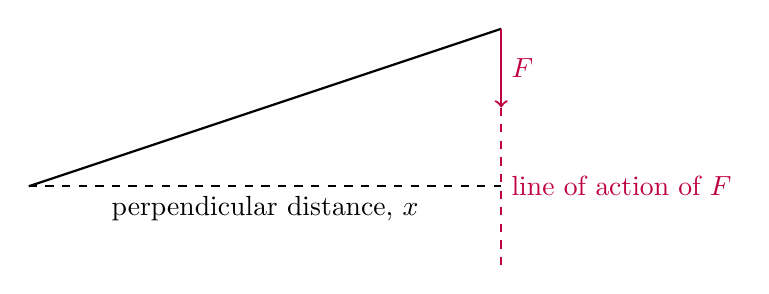
\begin{tikzpicture}
		\draw[thick] (0,0) -- (6,2);
		\draw[thick, purple, ->] (6,2) -- node[right]{$ F$}(6,1);
		\draw[thick, purple, dashed] (6,1) -- node[right] {line of action of $F$}(6,-1) ;
		\draw[thick, dashed] (0,0) -- node[below]{perpendicular distance, $x$} (6,0);

	\end{tikzpicture}
	$$\mathrm{moment} = Fx $$
\end{figure}

The conditions for equilibrium are:
\begin{enumerate}
	\item The sum of all the forces acting on the object must be zero.
	\item The sum of all the moments on an object must be zero.
\end{enumerate}

\fbox{\begin{minipage}[t]{\textwidth}
	\textbf{Example Question}

	A Tower Crane lifts a load into position. The load has a weight of \SI{4.0e4}{N} and the arm of the crane has a weight of \SI{1.2e5}{N}.

	Calculate the required weight of the counterweight and the force the tower must support. Assume the centre of mass of the arm is at its centre.

	\vspace{1cm}

		\begin{center}
		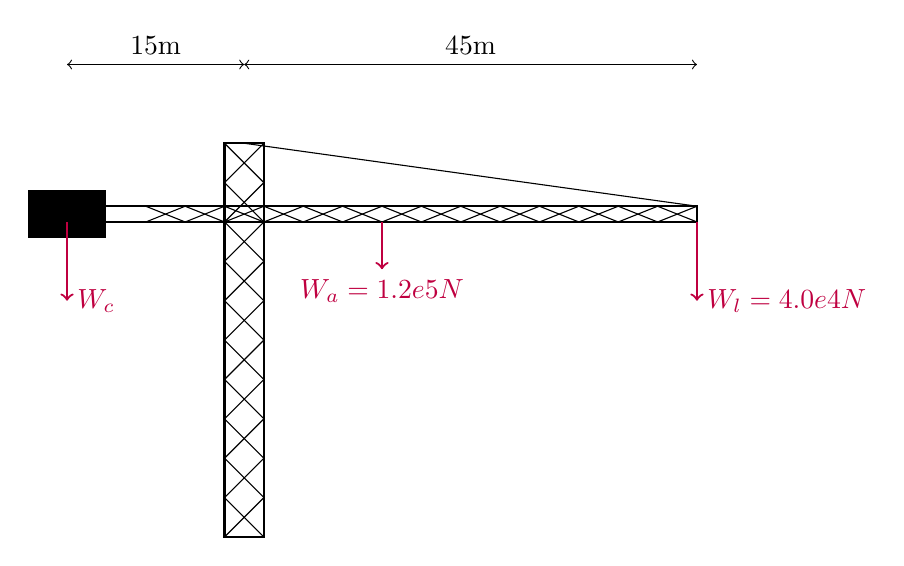
\begin{tikzpicture}
					\draw[thick] (2,0) rectangle (2.5,5);
					\draw[thick] (0,4) rectangle (8,4.2);
					\fill (-0.5,3.8) rectangle (.5,4.4);
					\draw(2.25,5) -- (8,4.2);
					\foreach \x in {0,1,...,13} {
						\draw (1+0.5*\x,4) -- (1.5+0.5*\x,4.2);
						\draw (1+0.5*\x,4.2) -- (1.5+0.5*\x,4);
					}
					\foreach \y in {0,1,...,9} {
						\draw (2,0+0.5*\y) -- (2.5,0.5+0.5*\y);
						\draw (2.5,0+0.5*\y) -- (2,0.5+0.5*\y);
					}
					\draw[purple, thick, ->] (8,4) -- (8,3) node[right]{$W_l=\SI{4.0e4}{N}$};
					\draw[purple, thick, ->] (4,4) -- (4,3.4) node[below]{$W_a=\SI{1.2e5}{N}$};
					\draw[purple, thick, ->] (0,4) -- (0,3) node[right]{$W_c$};
					\draw[<->] (0,6) -- node[above]{15m}(2.25,6);
					\draw[<->] (2.25,6) -- node[above]{45m}(8,6);
				\end{tikzpicture}
		\end{center}

		\textbf{Answer}

		We begin by taking moments around the tower of the crane. The weight of the arm, $W_a$, acts \SI{15}{m} from the tower so solving for moments gives:

		$$ 15W_c = 15W_a + 25W_l $$
		$$ W_c = \SI{4.2e5}{N} $$

		The sum of the downward forces must equal the reaction force of the tower so:

		$$ R = \SI{4.0e5}{N} $$



\end{minipage}}

\spec{(e) construct displacement-time and velocity-time graphs for uniformly accelerated motion}



\end{document}
